\chapter{Example Chapter Three: Some Notes About Table and Figure Formatting}


\noindent Tables and figures are a bit annoying. Especially in keeping with the formatting guidelines. Remember that table and figure text can be no smaller than font size 9, and no larger than 12. This means I re-rendered many of my figures in R to meet this criteria. Tables, at times, needed to be split or compressed to fit within the margins.

The figures and tables below are from another paper of mine that were published \autocite{rozelle_user_2026}. I would flag that LANDSCAPE ORIENTED TABLES MUST BE RENDERED IN PORTRAIT MODE. This is something that caught a few of the PhD candidates I spoke to, including myself. The current \LaTeX~ template manages this the way the graduate school wants it, but uses a less standard package to do so.

ChatGPT or Claude are great at helping to format tables and getting them to fit in a page until you can do it yourself, but I would recommend using the \texttt{threeparttable} package. It helps keep everything tidy, from caption to notes (see \ref{ch3:tab:table1}). Tables and figures in the appendix come from my dissertation \autocite{rozelle_measuring_2026}.

\section{Methods}

\subsection{Analytic approach}

Look, \LaTeX~ can do some cool formulas (one of my favorite things about it (see Equation \ref{eq:final_sri})! For an even more interesting equation, check Appendix \ref{appx:methods}.

\begin{equation}
    \label{eq:final_sri}
    y_{ik} = \beta_0 + \beta_{1}\text{Fees}_{i} + \beta_{2}\text{Rural}_{i} + \boldsymbol{\beta_{3}}\mathbf{F}_{i} + \beta_{4}\text{Services}_{i} + u_{g(k)} + \epsilon_{ik}
\end{equation}

\noindent In the equation, $y_{ik}$is the example outcome for stratum $k$.  In rhoncus, ante ornare laoreet dictum, nunc diam laoreet risus, sed elementum lacus tellus nec sapien. Integer malesuada ante at turpis pulvinar feugiat. Aenean fermentum tincidunt molestie. Integer pharetra mattis tortor vel auctor. Aenean finibus a felis sit amet rhoncus. Phasellus non lectus et enim aliquet fermentum et ut nunc. Curabitur tincidunt placerat gravida.

Sed molestie augue non laoreet tempus. Nulla sagittis lectus vitae enim congue, ac aliquet mi fringilla. Vivamus quis lobortis metus. Phasellus iaculis nibh augue, in molestie leo malesuada eu. Etiam ultricies elit est, sed commodo massa suscipit vitae. Fusce pellentesque sit amet neque blandit interdum. Nullam purus ipsum, vulputate et pharetra ut, rhoncus nec ante. Fusce risus lacus, hendrerit eu felis eu, suscipit mollis lorem. Morbi nec urna eu metus elementum tempor quis ut mi. Vivamus venenatis varius enim, eu volutpat tellus suscipit nec. Mauris vulputate sit amet diam et condimentum. Fusce eget volutpat elit. 

All facility-level regression coefficients (including the client-fee indicator and covariates) were assigned improper flat priors over $\mathbb{R}$. The model intercept was assigned a Student-t prior with three degrees of freedom, centered at the observed mean of the outcome. The standard deviation of the managing authority by facility-type random intercept, as well as the residual standard deviation, were assigned half Student-t priors with three degrees of freedom and scale 2.5 (Student-t(3, 0, 2.5), constrained to be non-negative).

All models were fit with cmdstanr via brms using 8,000 iterations (4,000 warmup) per chain across eight chains. Convergence was assessed using standard diagnostics (Rhat = 1.00 and effective sample sizes), alongside posterior predictive checks. All monitored parameters met these convergence thresholds (Rhat = 1.00).

\section{Results}

Look below at the landscape table here, which is a great table (see Table \ref{ch3:tab:table1}). If you write a dissertation, I hope your tables look this good.

\begin{landscape}
\begin{table}[H]
\begin{singlespace}
\centering
\begin{threeparttable}
    
\caption[Short caption for TOC, table with landscape]{This is a much longer caption, and I can include a few more details here if I want, or different text than what is in the TOC altogether}
\label{ch3:tab:table1}
\begin{tabular}{lcccccc}
\hline\hline
& \textbf{Afghanistan} & \textbf{Bangladesh} & \textbf{Ethiopia} & 
\textbf{Malawi} & \textbf{Nepal} & \textbf{Tanzania} \\
& (2018) & (2017) & (2021--22) & (2013--14) & (2021) & (2014--15) \\
\textbf{Number of facilities ($n$)} 
& 92 & 1{,}338 & 1{,}060 & 782 & 1{,}297 & 928 \\
\midrule

Facilities charging client fees (\%) 
& 75.0 & 37.2 & 78.8 & 38.5 & 30.9 & 91.8 \\

\textbf{Overall SRI (0--10)} 
& 7.70 & 4.56 & 6.23 & 6.00 & 5.90 & 5.53 \\

\quad{Basic amenities} 
& 8.99 & 5.14 & 6.41 & 6.84 & 6.46 & 5.49 \\

\quad{Basic equipment} 
& 8.42 & 8.17 & 8.54 & 7.94 & 9.26 & 7.66 \\

\quad{Infection prevention} 
& 7.15 & 5.97 & 7.48 & 7.08 & 5.34 & 6.53 \\

\quad{Diagnostic capacity} 
& 7.32 & 1.15 & 4.75 & 3.47 & 3.48 & 4.16 \\

\quad{Essential medicines} 
& 6.62 & 2.35 & 3.98 & 4.69 & 4.94 & 3.82 \\

\textbf{Funding source (\%)} & & & & & & \\
\quad Public & 37.0 & 97.1 & 63.0 & 61.8 & 15.0 & 68.9 \\
\quad Private & 22.8 & 0.2 & 5.3 & 6.5 & 11.2 & 46.9 \\
\quad Non-state/NGO & 13.0 & 9.0 & 23.0 & 35.9 & 73.6 & 34.7 \\

\textbf{Managing authority (\%)} & & & & & & \\
\quad Public & 34.8 & 96.8 & 77.3 & 58.2 & 96.8 & 82.2 \\
\quad Private-for-profit & 54.3 & 0.0 & 20.9 & 31.7 & 0.0 & 12.5 \\
\quad Private-nonprofit & 10.9 & 3.2 & 1.8 & 10.1 & 3.2 & 5.3 \\

\textbf{Facility type (\%)} & & & & & & \\
\quad Hospital & 89.1 & 15.2 & 29.0 & 8.4 & 21.9 & 10.7 \\
\quad Health centre & 10.9 & 60.5 & 46.8 & 86.4 & 0.0 & 36.2 \\
\quad Health post / dispensary & 0.0 & 24.3 & 24.2 & 5.1 & 32.1 & 53.1 \\

\textbf{Rural facilities (\%)} 
& 1.1 & 82.1 & 51.6 & 66.5 & 41.3 & 68.1 \\

\bottomrule
\end{tabular}

\begin{tablenotes}[flushleft]
\fontsize{9pt}{10.5pt}\selectfont
\item \textit{Notes:} In the \texttt{tablenotes} section, you can include some nicely aligned and formatted table notes. I kept these consistently size 9 so I didn't have to think about it.  
\end{tablenotes}

\end{threeparttable}
\end{singlespace}
\end{table}
\end{landscape}

 Proin venenatis mattis convallis. Morbi cursus pulvinar lorem, vel fringilla nibh bibendum sit amet. Phasellus ut lacus bibendum mi facilisis sodales. Pellentesque ultricies risus vitae viverra hendrerit. Fusce lobortis, dolor vel fringilla lobortis, tellus nibh ultricies lectus, quis placerat quam est a elit. Phasellus at quam finibus neque condimentum euismod sit amet nec est. Sed nec mollis nibh, a dapibus justo. Sed turpis lectus, lacinia quis sapien non, suscipit venenatis diam. Nunc facilisis ut arcu eu gravida. Sed felis sem, semper in sodales a, sodales a lacus. Sed lacinia nec nunc a ornare. Donec id nulla metus. Praesent viverra egestas justo, quis elementum dui posuere ac. Sed a condimentum velit, sit amet egestas eros. Nam iaculis, odio vel pharetra placerat, diam justo molestie sapien, sit amet fringilla massa magna id erat.

Nunc viverra rhoncus nulla, pretium interdum erat scelerisque quis. Cras ornare, libero et bibendum semper, quam elit accumsan tortor, sed efficitur libero ipsum non velit. Donec at justo suscipit, viverra arcu vestibulum, volutpat enim. If you're paying attention to this, I will reference the figure in the middle of the lorem ipsum paragraph. You should call me if you see this (see Figure \ref{ch3:fig:sri_heatmap}). Integer sed dapibus nunc. Nulla interdum nisl ligula, quis facilisis justo vestibulum et. Cras consequat egestas fringilla. Vestibulum nec commodo arcu, sit amet condimentum neque. Maecenas sed magna posuere, dignissim quam sit amet, euismod enim. Vivamus semper viverra turpis, eget viverra felis. Integer gravida molestie ex. Nam maximus et dolor a luctus. Integer bibendum, ante eu pellentesque pharetra, nibh ex condimentum ex, vitae eleifend dui lectus nec magna. Nulla sagittis faucibus eros ut tincidunt. Aenean commodo accumsan est, eget elementum nibh malesuada eget. Praesent tempor quam non lacus malesuada, ac sollicitudin enim sodales. Proin at enim elementum magna vulputate semper. 

\clearpage
\begin{landscape}
  
\begin{figure}[htbp]
  \centering
  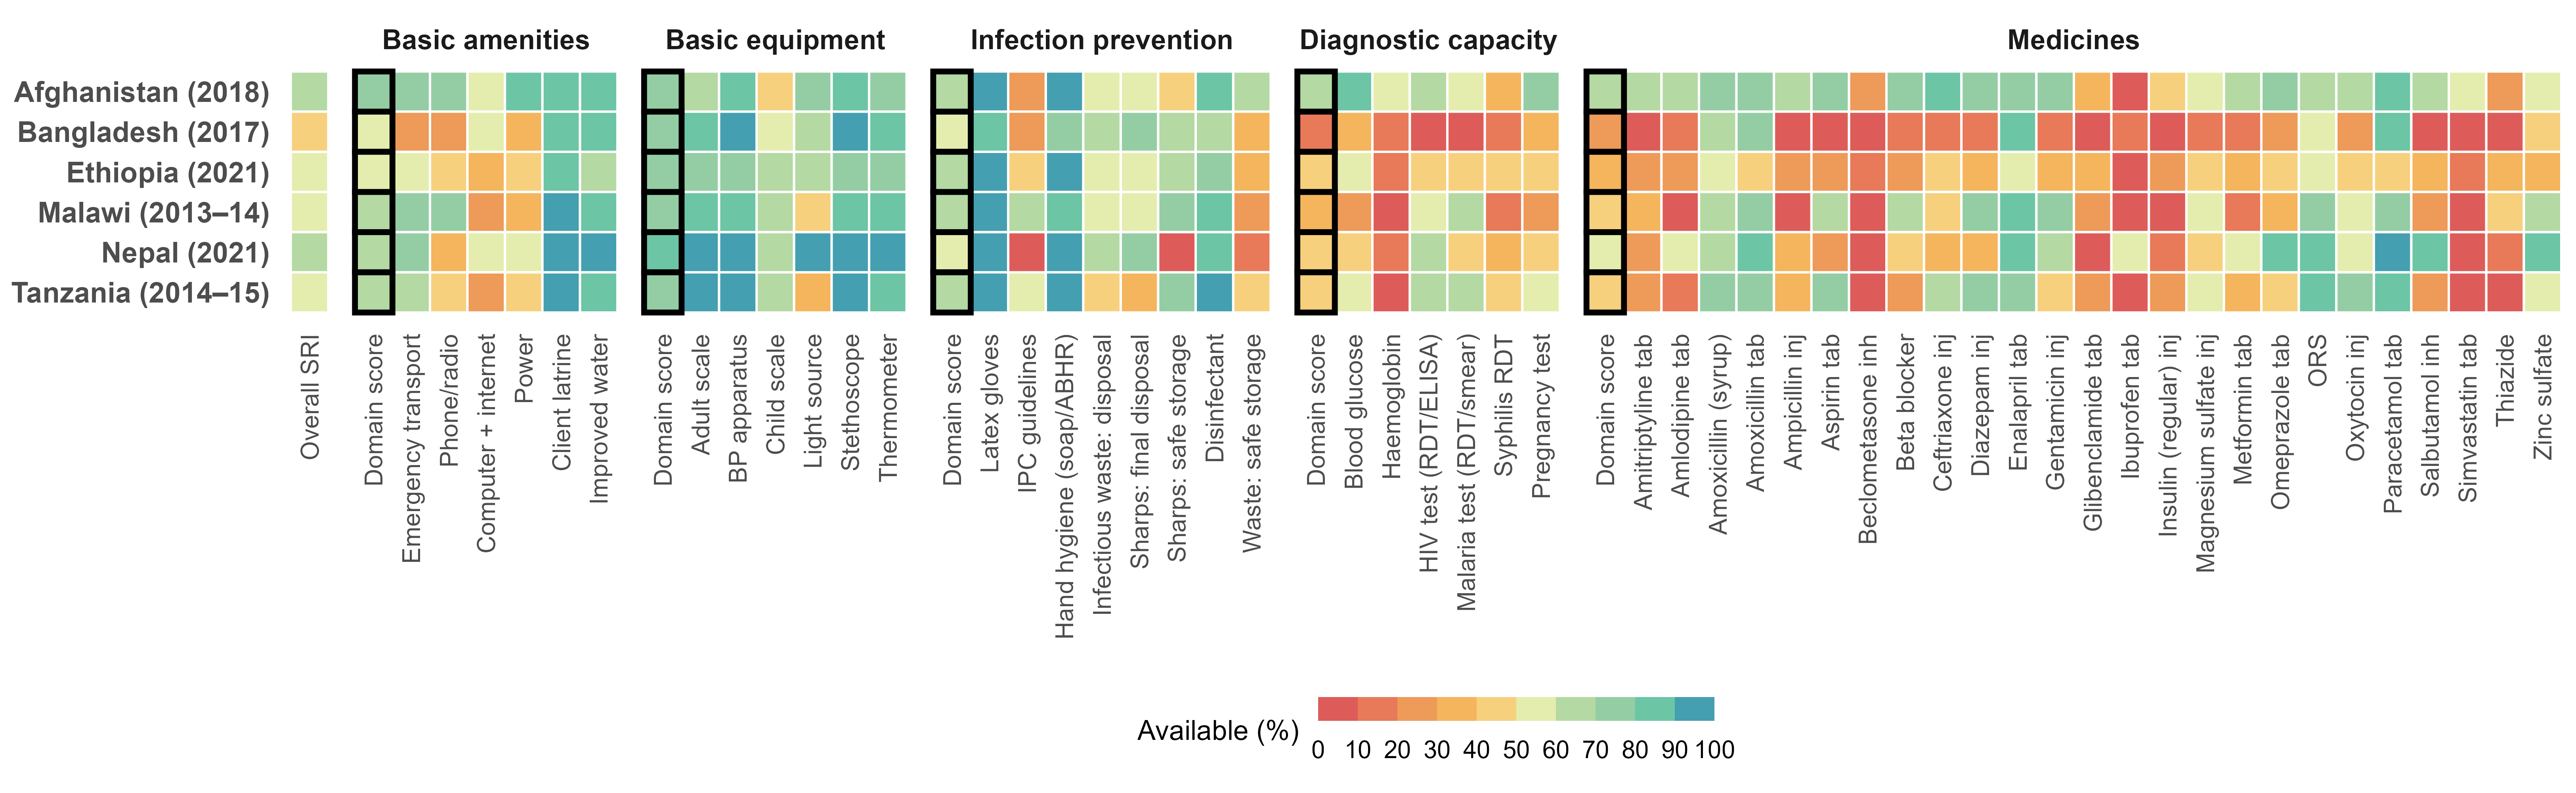
\includegraphics[width=9in]{images/figure1_sri_heatmap.png}
  \caption[Cross-country Service Readiness Index (SRI) profiles by domain and selected tracer items]{Cross-country Service Readiness Index (SRI) profiles by domain and selected tracer items. Domain scores are rescaled from 0--10 to 0--100; tracer items show the percentage of facilities with the item observed on the day of assessment. Higher values indicate greater readiness or item availability (see color bar).}
  \label{ch3:fig:sri_heatmap}
\end{figure}
\end{landscape}

 Vestibulum lacinia imperdiet massa. Praesent non massa blandit, bibendum dui eu, sodales arcu. Vestibulum scelerisque metus non tincidunt viverra. Orci varius natoque penatibus et magnis dis parturient montes, nascetur ridiculus mus. Morbi lacinia pretium arcu ut tincidunt. Etiam orci massa, efficitur id vehicula in, tincidunt ut eros. Vestibulum nec nulla vel metus varius efficitur in sit amet ipsum. Vestibulum rutrum elementum ullamcorper. Curabitur elit dui, interdum eu nibh id, congue suscipit lacus. Aenean velit lectus, mattis in odio ut, viverra pharetra tortor. Donec dapibus, tellus quis dictum aliquam, elit lacus dapibus eros, non consequat nunc orci quis odio. Vivamus ultricies convallis eros, sit amet sagittis velit consequat a. Fusce quis tortor sit amet ante bibendum pellentesque dignissim et diam.

Etiam semper rutrum enim elementum laoreet. Proin tristique sem metus, id sodales ante vulputate ut. Ut bibendum pulvinar nisi vitae condimentum. Pellentesque leo magna, semper eu dapibus sit amet, hendrerit non sapien. Morbi posuere facilisis urna, eget posuere quam porta non. Nam ac lacus diam. Suspendisse at quam elit. Nullam sagittis leo eget est vehicula mattis. 

\section{Discussion}

 Etiam semper rutrum enim elementum laoreet. Proin tristique sem metus, id sodales ante vulputate ut. Ut bibendum pulvinar nisi vitae condimentum. Pellentesque leo magna, semper eu dapibus sit amet, hendrerit non sapien. Morbi posuere facilisis urna, eget posuere quam porta non. Nam ac lacus diam. Suspendisse at quam elit. Nullam sagittis leo eget est vehicula mattis.

Proin venenatis mattis convallis. Morbi cursus pulvinar lorem, vel fringilla nibh bibendum sit amet. Phasellus ut lacus bibendum mi facilisis sodales. Pellentesque ultricies risus vitae viverra hendrerit. Fusce lobortis, dolor vel fringilla lobortis, tellus nibh ultricies lectus, quis placerat quam est a elit. Phasellus at quam finibus neque condimentum euismod sit amet nec est. Sed nec mollis nibh, a dapibus justo. Sed turpis lectus, lacinia quis sapien non, suscipit venenatis diam. Nunc facilisis ut arcu eu gravida. Sed felis sem, semper in sodales a, sodales a lacus. Sed lacinia nec nunc a ornare. Donec id nulla metus. Praesent viverra egestas justo, quis elementum dui posuere ac. Sed a condimentum velit, sit amet egestas eros. Nam iaculis, odio vel pharetra placerat, diam justo molestie sapien, sit amet fringilla massa magna id erat.

Nunc viverra rhoncus nulla, pretium interdum erat scelerisque quis. Cras ornare, libero et bibendum semper, quam elit accumsan tortor, sed efficitur libero ipsum non velit. Donec at justo suscipit, viverra arcu vestibulum, volutpat enim. Integer sed dapibus nunc. Nulla interdum nisl ligula, quis facilisis justo vestibulum et. Cras consequat egestas fringilla. Vestibulum nec commodo arcu, sit amet condimentum neque. Maecenas sed magna posuere, dignissim quam sit amet, euismod enim. Vivamus semper viverra turpis, eget viverra felis. Integer gravida molestie ex. Nam maximus et dolor a luctus. Integer bibendum, ante eu pellentesque pharetra, nibh ex condimentum ex, vitae eleifend dui lectus nec magna.





